\section{Decision Trees}

\begin{frame}{From Density-Based Clustering to Supervised Rules}
\begin{columns}[T]
\column{0.52\textwidth}
\begin{itemize}
  \item DBSCAN used local density to find structure without target labels.
  \pause
  \item Decision trees return to the supervised setting: each example has a target label.
  \pause
  \item A node is \textbf{pure} when its examples mostly belong to one class.
  \pause
  \item A node is \textbf{impure} when examples from different classes are mixed.
  \pause
  \item The key idea is to choose questions that reduce impurity.
\end{itemize}

\pause
\column{0.48\textwidth}
\centering
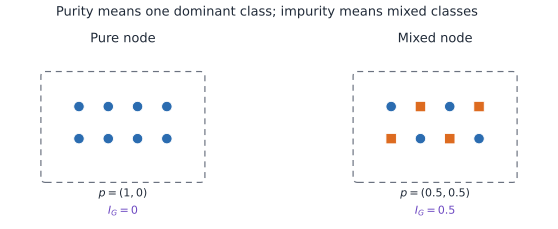
\includegraphics[width=\textwidth]{figures/decision_trees/decision_tree_purity_impurity.pdf}
\end{columns}
\end{frame}

\begin{frame}{Why Decision Trees?}
\begin{columns}[T]
\column{0.52\textwidth}
\begin{itemize}
  \item Input: examples $x_1,\dots,x_n \in \mathbb{R}^d$ with targets $y_1,\dots,y_n$.
  \pause
  \item Output: a tree of decision rules and predictions at the leaves.
  \pause
  \item The method is useful because the learned rules can be inspected directly.
\end{itemize}

\pause
\column{0.48\textwidth}
\textbf{Typical uses}
\begin{itemize}
  \item interpretable classification,
  \pause
  \item tabular data modeling,
  \pause
  \item feature interaction discovery,
  \pause
  \item base learners for random forests and boosting.
\end{itemize}
\end{columns}

\pause
\begin{rlintuition}
k-NN predicts from nearby examples. A decision tree predicts by routing an example through learned questions.
\end{rlintuition}
\end{frame}

\begin{frame}{Formal Setup}
\begin{columns}[T]
\column{0.52\textwidth}
\begin{itemize}
  \item Let
  \[
    D=\{(x_i,y_i)\}_{i=1}^{n},
    \qquad
    x_i \in \mathbb{R}^d.
  \]
  \pause
  \item For classification, assume
  \[
    y_i \in \{1,\dots,C\}.
  \]
  \pause
  \item A tree partitions the feature space into regions.
  \pause
  \item Each leaf predicts one class from the training examples that reach that leaf.
\end{itemize}

\pause
\column{0.48\textwidth}
\centering
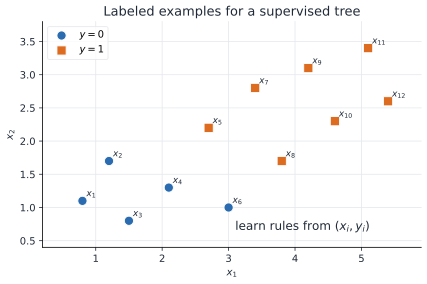
\includegraphics[width=\textwidth]{figures/decision_trees/decision_tree_formal_setup.pdf}
\end{columns}
\end{frame}

\begin{frame}{One Split Rule}
\begin{columns}[T]
\column{0.53\textwidth}
\begin{itemize}
  \item At one node, the tree considers a feature $j$ and a threshold $t$.
  \pause
  \item The split sends examples to
  \begin{equation}
    \begin{aligned}
      D_L &= \{(x_i,y_i)\in D_m : x_{ij} \leq t\},\\
      D_R &= \{(x_i,y_i)\in D_m : x_{ij} > t\}.
    \end{aligned}
    \label{eq:tree-split}
  \end{equation}
  \pause
  \item Here $D_m$ is the set of training examples that reached the current node.
\end{itemize}

\pause
\column{0.47\textwidth}
\centering
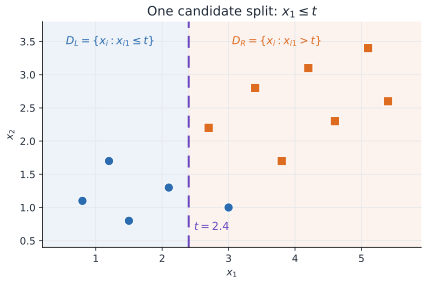
\includegraphics[width=\textwidth]{figures/decision_trees/decision_tree_split_rule.pdf}
\end{columns}
\end{frame}

\begin{frame}{Class Proportions in a Node}
\begin{itemize}
  \item Let $D_m$ be the examples at node $m$ and let $n_m=|D_m|$.
  \pause
  \item The class proportion for class $c$ is
  \begin{equation}
    p_{mc}
    =
    \frac{1}{n_m}
    \sum_{(x_i,y_i)\in D_m}\mathbf{1}\{y_i=c\}.
    \label{eq:node-class-proportion}
  \end{equation}
  \pause
  \item A pure node has all examples from one class.
  \pause
  \item A mixed node contains examples from several classes.
\end{itemize}
\end{frame}

\begin{frame}{Impurity}
\begin{columns}[T]
\column{0.52\textwidth}
\begin{itemize}
  \item A tree chooses splits using a measure of node impurity.
  \pause
  \item One common choice is Gini impurity:
  \begin{equation}
    I_G(D_m)
    =
    1-\sum_{c=1}^{C}p_{mc}^{2}.
    \label{eq:gini-impurity}
  \end{equation}
  \pause
  \item Another common choice is entropy:
  \begin{equation}
    I_H(D_m)
    =
    -\sum_{c=1}^{C}p_{mc}\log_2 p_{mc}.
    \label{eq:entropy-impurity}
  \end{equation}
\end{itemize}

\pause
\column{0.48\textwidth}
\centering
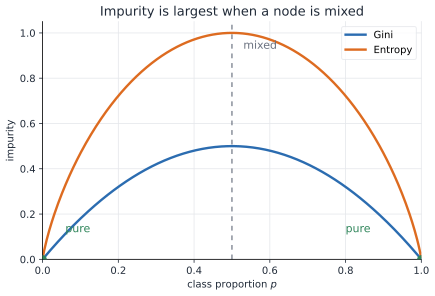
\includegraphics[width=\textwidth]{figures/decision_trees/decision_tree_impurity_curves.pdf}
\end{columns}
\end{frame}

\begin{frame}{Split Objective}
\begin{itemize}
  \item A good split reduces impurity.
  \pause
  \item For a candidate split $(j,t)$, define
  \begin{equation}
    \Delta I(j,t)
    =
    I(D_m)
    -
    \frac{|D_L|}{|D_m|}I(D_L)
    -
    \frac{|D_R|}{|D_m|}I(D_R).
    \label{eq:impurity-decrease}
  \end{equation}
  \pause
  \item The tree chooses the split with the largest impurity decrease.
  \pause
  \item This is a greedy local decision, not a global search over all possible trees.
\end{itemize}
\end{frame}

\begin{frame}{Searching for a Split}
\centering
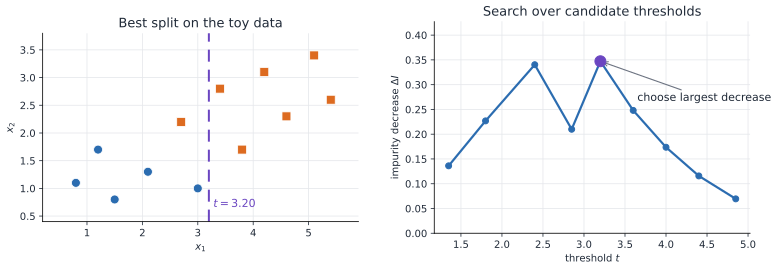
\includegraphics[width=0.94\textwidth]{figures/decision_trees/decision_tree_split_gain.pdf}

\vspace{0.35em}
\begin{itemize}
  \item For each feature, try candidate thresholds.
  \pause
  \item Compute the weighted child impurity.
  \pause
  \item Keep the split with the largest decrease $\Delta I$.
\end{itemize}
\end{frame}

\begin{frame}{Worked Numerical Example}
\small
\begin{itemize}
  \item Suppose a node contains $10$ examples with class counts
  \[
    n_{m1}=6,
    \qquad
    n_{m2}=4.
  \]
  \pause
  \item Then
  \[
    p_{m1}=0.6,
    \qquad
    p_{m2}=0.4.
  \]
  \pause
  \item The Gini impurity is
  \[
    I_G(D_m)=1-0.6^2-0.4^2=0.48.
  \]
  \pause
  \item The node is mixed because both classes are present.
\end{itemize}
\end{frame}

\begin{frame}{Worked Numerical Example: Split}
\small
\begin{itemize}
  \item A candidate split sends $5$ examples left and $5$ examples right.
  \pause
  \item Left child counts:
  \[
    (5,0)
    \quad\Rightarrow\quad
    I_G(D_L)=1-1^2-0^2=0.
  \]
  \pause
  \item Right child counts:
  \[
    (1,4)
    \quad\Rightarrow\quad
    I_G(D_R)=1-0.2^2-0.8^2=0.32.
  \]
  \pause
  \item Therefore
  \[
    \Delta I
    =
    0.48-\frac{5}{10}(0)-\frac{5}{10}(0.32)
    =
    0.32.
  \]
\end{itemize}
\end{frame}

\begin{frame}{Prediction}
\begin{columns}[T]
\column{0.53\textwidth}
\begin{itemize}
  \item After the tree is trained, a new example is routed from the root to one leaf.
  \pause
  \item Each internal node applies one split rule.
  \pause
  \item For classification, the leaf prediction is usually the majority class:
  \begin{equation}
    \hat{y}
    =
    \arg\max_{c\in\{1,\dots,C\}} p_{mc}.
    \label{eq:tree-majority-prediction}
  \end{equation}
\end{itemize}

\pause
\column{0.47\textwidth}
\centering
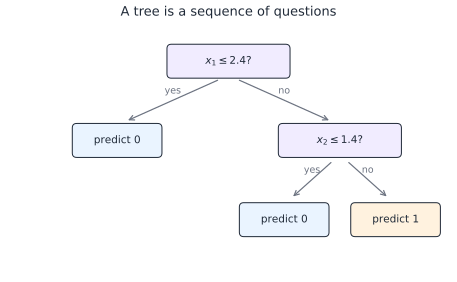
\includegraphics[width=\textwidth]{figures/decision_trees/decision_tree_prediction.pdf}
\end{columns}
\end{frame}

\begin{frame}{Decision Regions}
\centering
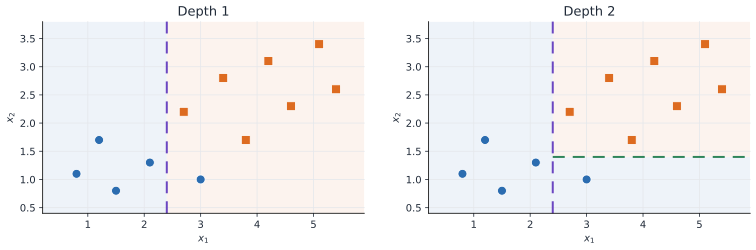
\includegraphics[width=0.92\textwidth]{figures/decision_trees/decision_tree_regions.pdf}

\vspace{0.35em}
\begin{itemize}
  \item Each split creates an axis-aligned cut in the feature space.
  \pause
  \item Deeper trees combine many cuts into more detailed decision regions.
\end{itemize}
\end{frame}

\begin{frame}{Basic Tree-Growing Algorithm}
\begin{enumerate}
  \item Start with all training examples at the root node.
  \pause
  \item Search over candidate feature-threshold splits.
  \pause
  \item Choose the split with the largest impurity decrease.
  \pause
  \item Recursively repeat the same procedure in each child node.
  \pause
  \item Stop when a stopping condition is reached.
\end{enumerate}
\end{frame}

\begin{frame}{Stopping Conditions}
\begin{itemize}
  \item Stop if the node is already pure.
  \pause
  \item Stop if the node contains too few examples.
  \pause
  \item Stop if the maximum depth is reached.
  \pause
  \item Stop if no candidate split gives enough impurity decrease.
  \pause
  \item These conditions control the complexity of the learned tree.
\end{itemize}
\end{frame}

\begin{frame}{Overfitting}
\centering
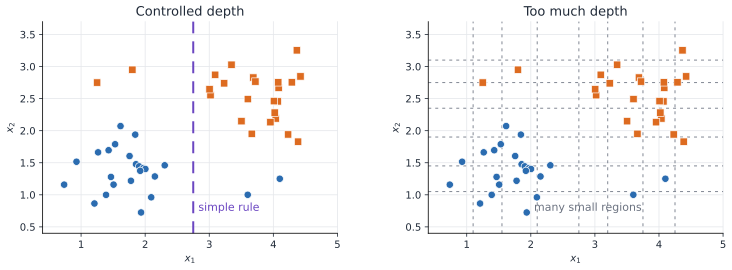
\includegraphics[width=0.92\textwidth]{figures/decision_trees/decision_tree_overfitting.pdf}

\vspace{0.35em}
\begin{itemize}
  \item A very deep tree can create small regions that fit training noise.
  \pause
  \item Limiting depth, minimum leaf size, or pruning reduces this risk.
\end{itemize}
\end{frame}

\begin{frame}{Regression Trees}
\begin{itemize}
  \item Decision trees can also be used for regression.
  \pause
  \item Now the target is continuous:
  \[
    y_i \in \mathbb{R}.
  \]
  \pause
  \item A common split objective minimizes squared error inside the child nodes.
  \pause
  \item The prediction at a leaf is the mean target value of training examples in that leaf:
  \begin{equation}
    \hat{y}
    =
    \frac{1}{n_m}\sum_{(x_i,y_i)\in D_m} y_i.
    \label{eq:regression-tree-leaf-mean}
  \end{equation}
\end{itemize}
\end{frame}

\begin{frame}{Decision Trees Versus k-NN}
\begin{columns}[T]
\column{0.5\textwidth}
\textbf{k-NN}
\begin{itemize}
  \item stores the training examples,
  \pause
  \item predicts using distances at test time,
  \pause
  \item depends strongly on scaling,
  \pause
  \item gives local predictions from neighbors.
\end{itemize}

\pause
\column{0.5\textwidth}
\textbf{Decision trees}
\begin{itemize}
  \item compress training data into rules,
  \pause
  \item predict by following a path,
  \pause
  \item handle feature interactions through splits,
  \pause
  \item can overfit when grown too deeply.
\end{itemize}
\end{columns}
\end{frame}

\begin{frame}{When Decision Trees Work and When They Fail}
\begin{columns}[T]
\column{0.5\textwidth}
\textbf{Trees often work well when}
\begin{itemize}
  \item the data is tabular,
  \pause
  \item rules or thresholds are meaningful,
  \pause
  \item interpretability matters,
  \pause
  \item features interact in non-linear ways.
\end{itemize}

\pause
\column{0.5\textwidth}
\textbf{Trees can fail when}
\begin{itemize}
  \item the tree grows too deep,
  \pause
  \item small data changes alter the splits,
  \pause
  \item the best boundary is smooth and oblique,
  \pause
  \item the training labels contain much noise.
\end{itemize}
\end{columns}
\end{frame}

\begin{frame}{Summary}
\begin{itemize}
  \item A decision tree predicts by routing examples through feature-threshold questions.
  \item Each split partitions the current node into left and right child nodes.
  \item Classification trees choose splits by reducing impurity such as Gini impurity or entropy.
  \item Leaf predictions are usually majority classes for classification and means for regression.
  \item Tree depth and stopping rules control the tradeoff between underfitting and overfitting.
\end{itemize}
\end{frame}

\begin{frame}{Lab Connection}
\begin{itemize}
  \item Implement the computational core of a classification tree with NumPy: class counts, impurity, split search, and prediction.
  \item Compare shallow and deep trees on a tabular classification dataset.
  \item Report how maximum depth and minimum leaf size change training and validation accuracy.
  \item Explain one learned path from root to leaf in plain language.
\end{itemize}
\end{frame}
